\documentclass[11pt]{article}
\usepackage{bm}
\usepackage{stmaryrd}
\usepackage{graphicx}
\usepackage{hyperref}
\usepackage[utf8]{inputenc}
\usepackage{amsmath,amsthm,amsfonts,amssymb,amscd}
\usepackage{tikz}
\usepackage{xeCJK}
\usepackage{physics}
\usepackage{multirow,booktabs}
% \usepackage[table]{xcolor}
\usepackage{fullpage}
\usepackage{lastpage}
\usepackage{unicode-math}
\usepackage{enumitem}
\usepackage{fancyhdr}
\usepackage{mathrsfs}
\usepackage{wrapfig}
\usepackage{setspace}
\usepackage{calc}
\usepackage{multicol}
\usepackage{cancel}
\usepackage[retainorgcmds]{IEEEtrantools}
\usepackage[margin=3cm]{geometry}
\usepackage{amsmath}
\DeclareMathAlphabet{\mathcal}{OMS}{cmsy}{m}{n}
\let\mathbb\relax
\DeclareMathAlphabet{\mathbb}{U}{msb}{m}{n}
\newlength{\tabcont}
\setlength{\parindent}{0.0in}
\setlength{\parskip}{0.05in}
\usepackage{empheq}
\usepackage{framed}
\usepackage[most]{tcolorbox}
\usepackage{xcolor}
\linespread{1.2}
\graphicspath{{./}}
\setCJKmainfont[AutoFakeBold = 3, AutoFakeSlant = 4]{BiauKaiTC}
\colorlet{shadecolor}{orange!15}
\parindent 0in
\parskip 12pt
\geometry{margin=1in, headsep=0.25in}
\graphicspath{{./}}
\theoremstyle{definition}
\newtheorem{thr}{Theorem}
\newtheorem{lma}{Lemma}
\newtheorem{defn}{Definition}
\newtheorem{reg}{Rule}
\newtheorem{exer}{Exercise}
\newtheorem{note}{Note}
\newtheorem{asmp}{Assumption}
\newcommand*\diff{\mathop{}\!\mathrm{d}}
\begin{document}
\setcounter{section}{0}
\title{Title}

\thispagestyle{empty}
\begin{center}
  {\large \bf HTML HW4} \\ 
  B12901022 廖冠豪
\end{center}
\section*{5}
By definition of the Hessian we have
\begin{align*}
  A_E(\vb{w})_{ij} = \frac{\partial^2 }{\partial w_i\partial w_j}E_{in}(\vb{w}) \\ 
\end{align*}
\begin{align*}
  \pdv{E_{in}(\vb{w})}{w_i} &= \frac{1}{N}\sum_{n = 1}^N\frac{\exp(-y_n\vb{w}^T\vb{x}_n)(-y_n{{x}_n}_i)}{1 + \exp(-y_n{w}^T\vb{x}_n)} \\ 
\end{align*}
\begin{align*}
  \pdv{}{w_j}\left(\pdv{E_{in}(\vb{w})}{w_i}\right) &= \frac{1}{N}\sum^N_{n = 1}\frac{(\exp(-y_n\vb{w}^T\vb{x}_n)({\vb{x}_n}_i{\vb{x}_n}_j))(1 + \exp(-y_n\vb{w}^T\vb{x}_n)) - {\exp(-y_n\vb{w}^T\vb{x}_n)}^2({x_n}_i{x_n}_j)}{(1 + \exp(-y_n\vb{w}^T\vb{x}_n))^2} \\ 
  &=\frac{1}{N}\sum^N_{n=1} \frac{\exp(-y_n\vb{w}^T\vb{x}_n)}{(1 + \exp(-y_n\vb{w}^T\vb{x}_n))^2}{x_n}_i{x_n}_j \\ 
  &= \frac{1}{N}\sum^N_{n=1} \frac{1}{1 + \exp(-y_n\vb{w}^T\vb{x}_n)}\frac{1}{1 + \exp(y_n\vb{x}^T\vb{x}_n)}{x_n}_i{x_n}_j \\ 
  &= \frac{1}{N}\sum^N_{n = 1}h_t(\vb{x}_n)h_t(-\vb{x}_n){x_n}_i{x_n}_j \\ 
\end{align*}
(${x_n}_i$ is the i-th element of the $\vb{x}_n$, and is the same as $X_{ji}$)
For a N by d matrix $X$ and a N by N diagonal matrix $D$, we have
\begin{align*}
  {(X^TDX)}_{ij} = \sum^N_{n = 1}D_{nn}X_{ni}X_{nj}
\end{align*}
By comparing the expressions, we can obtain
\begin{align*}
  D_{ij} = 
  \begin{cases}
    0 & i \neq j\\
    \frac{1}{N}h_t(\vb{x}_n)h_t(-\vb{x}_n) & i = j\\
  \end{cases}
\end{align*}
\newpage 
\section*{6}
\textbf{In this problem, we use ${w_j}_i$ to denote the i-th element of $\vb{w}_j$, which is the same as $W_{ij}$}\\
Since $E_{\text{in}}$ is minmized with SGD, we know that
\[
  \text{V}_{ij} = -\pdv{}{{w_j}_i}\text{err}(W, \vb{x}, y)
\]
\begin{align*}
  \pdv{}{{w_j}_i}\text{err}(W, \vb{x}, y) &= -\frac{1}{h_y(\vb{x})}\pdv{h_y(\vb{x})}{{w_j}_i} \\ 
  &= -\frac{1}{h_y(\vb{x})}\frac{\llbracket y = i\rrbracket\exp(\vb{w}_y^T\vb{x})(\sum^K_{k = 1}\exp(\vb{w}_k^T\vb{x}))x_j- \exp(\vb{w}_y^T\vb{x})\exp(\vb{w}_i^T\vb{x})x_j}{\left(\sum^K_{k = 1}\exp(\vb{w}_k^T\vb{x})\right)^2 } \\ 
  &= -\frac{1}{h_y(\vb{x})}\frac{(\llbracket y = i\rrbracket - \exp(\vb{w}_i^T\vb{x}))\exp(\vb{w}_y^T\vb{x})x_j}{(\sum^K_{k = 1}\exp(\vb{w}_k^T\vb{x}))^2} \\ 
  &= -(\llbracket y = i\rrbracket - \frac{\exp(\vb{w}_i^T\vb{x})}{\sum^K_{k = 1}\exp(\vb{w}_k^T\vb{x})})x_j \\ 
  &= (h_i(\vb{x}) - \llbracket y = i\rrbracket)x_j
\end{align*}
Notice that 
\[
  (\vb{x}_n\cdot\vb{u}^T)_{ij} = x_ju_i
\]
Hence by comparing the expressions, $\vb{u}$ is given by
\[
  u_i = -h_i(\vb{x}_n) + \llbracket y_n = i\rrbracket
\]
\newpage 
\section*{7}
For MLR , we know that $\sum^N_{n = 1}\text{err}(\text{W}, \vb{x}, y)$ is minimized at its optimal solution, $(\vb{w}_1^\star, \vb{w}_2^\star)$. \\ 
Also
\begin{align*}
  \sum^N_{n = 1} \text{err}(\text{W}, \vb{w}, y) &= \sum^N_{n = 1} \ln\left(\frac{\exp(\vb{w}_{y_n}^T \vb{x}_n)}{\exp(\vb{w}_1^T \vb{x}_n) + \exp(\vb{w}_2^T \vb{x}_n)}\right) \\ 
  &= 
  \begin{cases}
    - \sum^N_{n = 1} \ln\left(1 + \exp((\vb{w}_2^T - \vb{w}_1^T) \vb{x}_n)\right) & \text{if } y_n = 1, \\[10pt]
    - \sum^N_{n = 1} \ln\left(1 + \exp((\vb{w}_1^T - \vb{w}_2^T) \vb{x}_n)\right) & \text{if } y_n = 2
  \end{cases} \\ 
  &= -\sum^N_{n = 1}\ln\left(1 +\exp(-y^\prime_n(\vb{w}_2 - \vb{w}_1)^T\vb{x}_n)\right)
\end{align*} 
For logistic regression
\begin{align*}
  E_{\text{in}}(\vb{w}) &= -\frac{1}{N}\sum^N_{n = 1}\ln\left(1 +\exp(-y^\prime_n\vb{w}^T\vb{x}_n)\right)
\end{align*}
By comparing the expressions, we see that $E_{\text{in}}(\vb{w})$ is minimized with
\[
  \vb{w}_{lr} = \vb{w}_2^\star - \vb{w}_1^\star
\]
Hence this is the optimal solution to the logistic regression.
\newpage
\section*{8}
The linear hypothesis that mimizes $E_{\text{in}}$ is the line that passes $(x_1, f(x_1))$ and $(x_2, f(x_2))$. \\ 
Hence
\begin{align*}
  g(x) &= f(x_1) + \frac{f(x_2) - f(x_1)}{x_2 - x_1}(x - x_1) \\ 
  &= -2(x_1 + x_2)x + 2x_1x_2 + 1
\end{align*}
For such a hypothesis, $E_{\text{in}} = 0$. \\ 
$E_{\text{out}}$ is given by
\begin{align*}
  E_{\text{out}} &= \int_0^1(g(x) - f(x))^2\diff x \\ 
  &= \int_0^1 \left(2x_1x_2 -2(x_1 + x_2)x + 2x^2\right)^2\diff x \\
\end{align*}
\begin{align*}
  \mathbb{E}_\mathcal{D}(|E_{\text{in}} - E_{\text{out}}|) &= \int^1_0\int^1_0|E_{\text{out}}|\diff x_1\diff x_2\quad(E_{\text{in}} = 0) \\ 
  &= \int^1_0\int^1_0\int^1_0\left(2x_1x_2 -2(x_1 + x_2)x + 2x^2\right)^2\diff x\diff x_1\diff x_2 \\ 
  &= \frac{2}{15}
\end{align*}
  % &= \int_0^1 4(x^4 + (x_1 + x_2)^2x^2 + x_1^2x_2^2 - 2x_1x_2(x_1 + x_2)x + 2x_1x_2x^2 - 2(x_1 + x_2)x^3)\diff x \\ 
  % &= \frac{4}{5} + \frac{1}{3}(x_1 + x_2)^2 + x_1^2x_2^2 - 2x_1x_2(x_1 + x_2) + \frac{2}{3}x_1x_2 - \frac{1}{2}(x_1 + x_2) \\
  % &= \frac{4}{5} + \frac{1}{3}(x_1^2 + x_2^2) + x_1x_2 + x_1^2x_2^2 - 2x_1^2x_2 - 2x_1x_2^2 - \frac{1}{2}(x_1 + x_2)
\newpage 
\section*{9}
Let
\begin{align*}
  \tilde{\text{X}} = \text{X} + \Epsilon
\end{align*}
Where
\begin{align*}
  \Epsilon = 
  \begin{bmatrix}
    | & \dots & | \\
    \epsilon &\dots&\epsilon \\
    | & \dots & | \\
  \end{bmatrix}
\end{align*}
\begin{align*}
  \text{X}_h^T\text{X}_h &= 
  \begin{bmatrix}
    \text{X}^T & \tilde{\text{X}}^T
  \end{bmatrix}
  \begin{bmatrix}
    \text{X} \\ 
    \tilde{X} \\
  \end{bmatrix} \\
  &= \text{X}^T\text{X} +  \tilde{\text{X}}^T\tilde{\text{X}} \\ 
  &= 2\text{X}^T\text{X} + \Epsilon^T\text{X} + \text{X}^T\Epsilon + \Epsilon^T\Epsilon
\end{align*}
Therefore 
\begin{align*}
  \mathbb{E}[\text{X}_h^T\text{X}_h] &= \mathbb{E}[2\text{X}^T\text{X} + \Epsilon^T\text{X} + \text{X}^T\Epsilon + \Epsilon^T\Epsilon] \\ 
  &= 2\text{X}^T\text{X} + \mathbb{E}[\Epsilon^T]\text{X} + \text{X}^T\mathbb{E}[\Epsilon] + \mathbb{E}[\Epsilon^T\Epsilon]
\end{align*}
Since $\epsilon$ is generated i.i.d. from a normal distribution with variance $\sigma^2$, we have
\begin{align*}
  \mathbb{E}[\Epsilon^T] &= \text{O}_{(d + 1)\times N} \\
  \mathbb{E}[\Epsilon] &= \text{O}_{N\times(d + 1)} \\ 
  \mathbb{E}[\Epsilon^T\Epsilon] &= N\sigma^2\text{I}_{d + 1}
\end{align*}
Hence 
\begin{align*}
  \mathbb{E}[\text{X}_h^T\text{X}_h] = 2\text{X}^T\text{X} + N\sigma^2\text{I}_{d + 1}
\end{align*}
So $(\alpha, \beta) = (2, N)$
\newpage
\section*{10}
Figure: \\
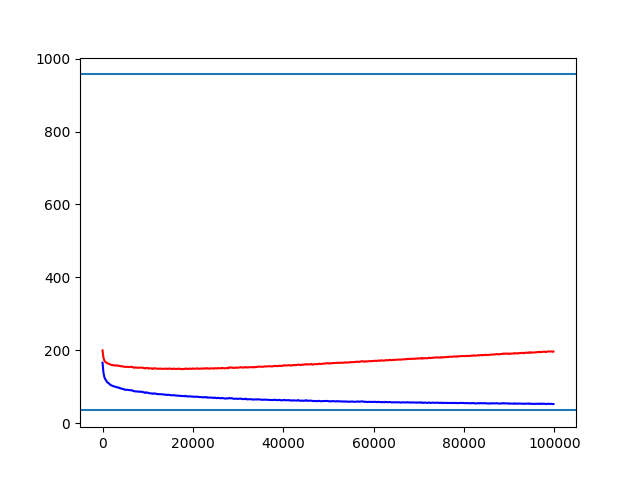
\includegraphics[width = \textwidth]{P10_fig2.png} \\
The horizontal light-blue lines at top and bottom are the average $E_{\text{out}}(\vb{w}_{lin})$ and $E_{\text{in}}(\vb{w}_{lin})$ respectively. \\ 
The red curve is the average $E_{\text{out}}(\vb{w}_t)$, and the dark-blue curve is the average $E_{\text{in}}(\vb{w}_t)$. \\  
The horizontal axis represents $t$ in the SGD process. \\ 
Findings: \\ 
First we can see that compared with the average values of linear regression, the $E_{\text{in}}$ of SGD is slightly larger, and the $E_{\text{out}}$ of SGD is significantly lower. This implies that SGD is probably a better approach compared with directly computing the weight vector in this case. \\ 
We see that starting from about $200$ at $t = 0$, $E_{\text{in}}(\vb{w}_t)$ decreases monotonically as $t$ increases. This is as expected, since the model can fit the $N = 64$ training data vectors better after more iterations. \\ 
We also see that as $t$ increases, $E_{\text{out}}(\vb{w}_t)$ first decreases slightly, after reaching its minimum at small $t$ (around 0), it begins to increase slowly. At the end of iterations $t = 100000$, $E_{\text{out}}(\vb{w}_t)$ is approximately at the same level as when the iteration started. A possible cause for this phenomenon is that at the very beginning of the SGD process, $E_{\text{out}}$ decreases because some information about the data set is learned by the algorithm. But as $t$ increases, the weight vector gets more biased by the $N = 64$ training data vectors, and its ability to classify the entire data set is compromised, hence the increasing $E_{\text{out}}$. This also means that a large number of iterations may not be meaningful or beneficial in this learning problem, since most iterations result in the increase of $E_\text{out}$. Moreover, there is no improve in $E_\text{out}$ at the end of the $100000$ iterations compared with at the beginning, when little "learning" is done. \\ 
Code snapshot: \\ 
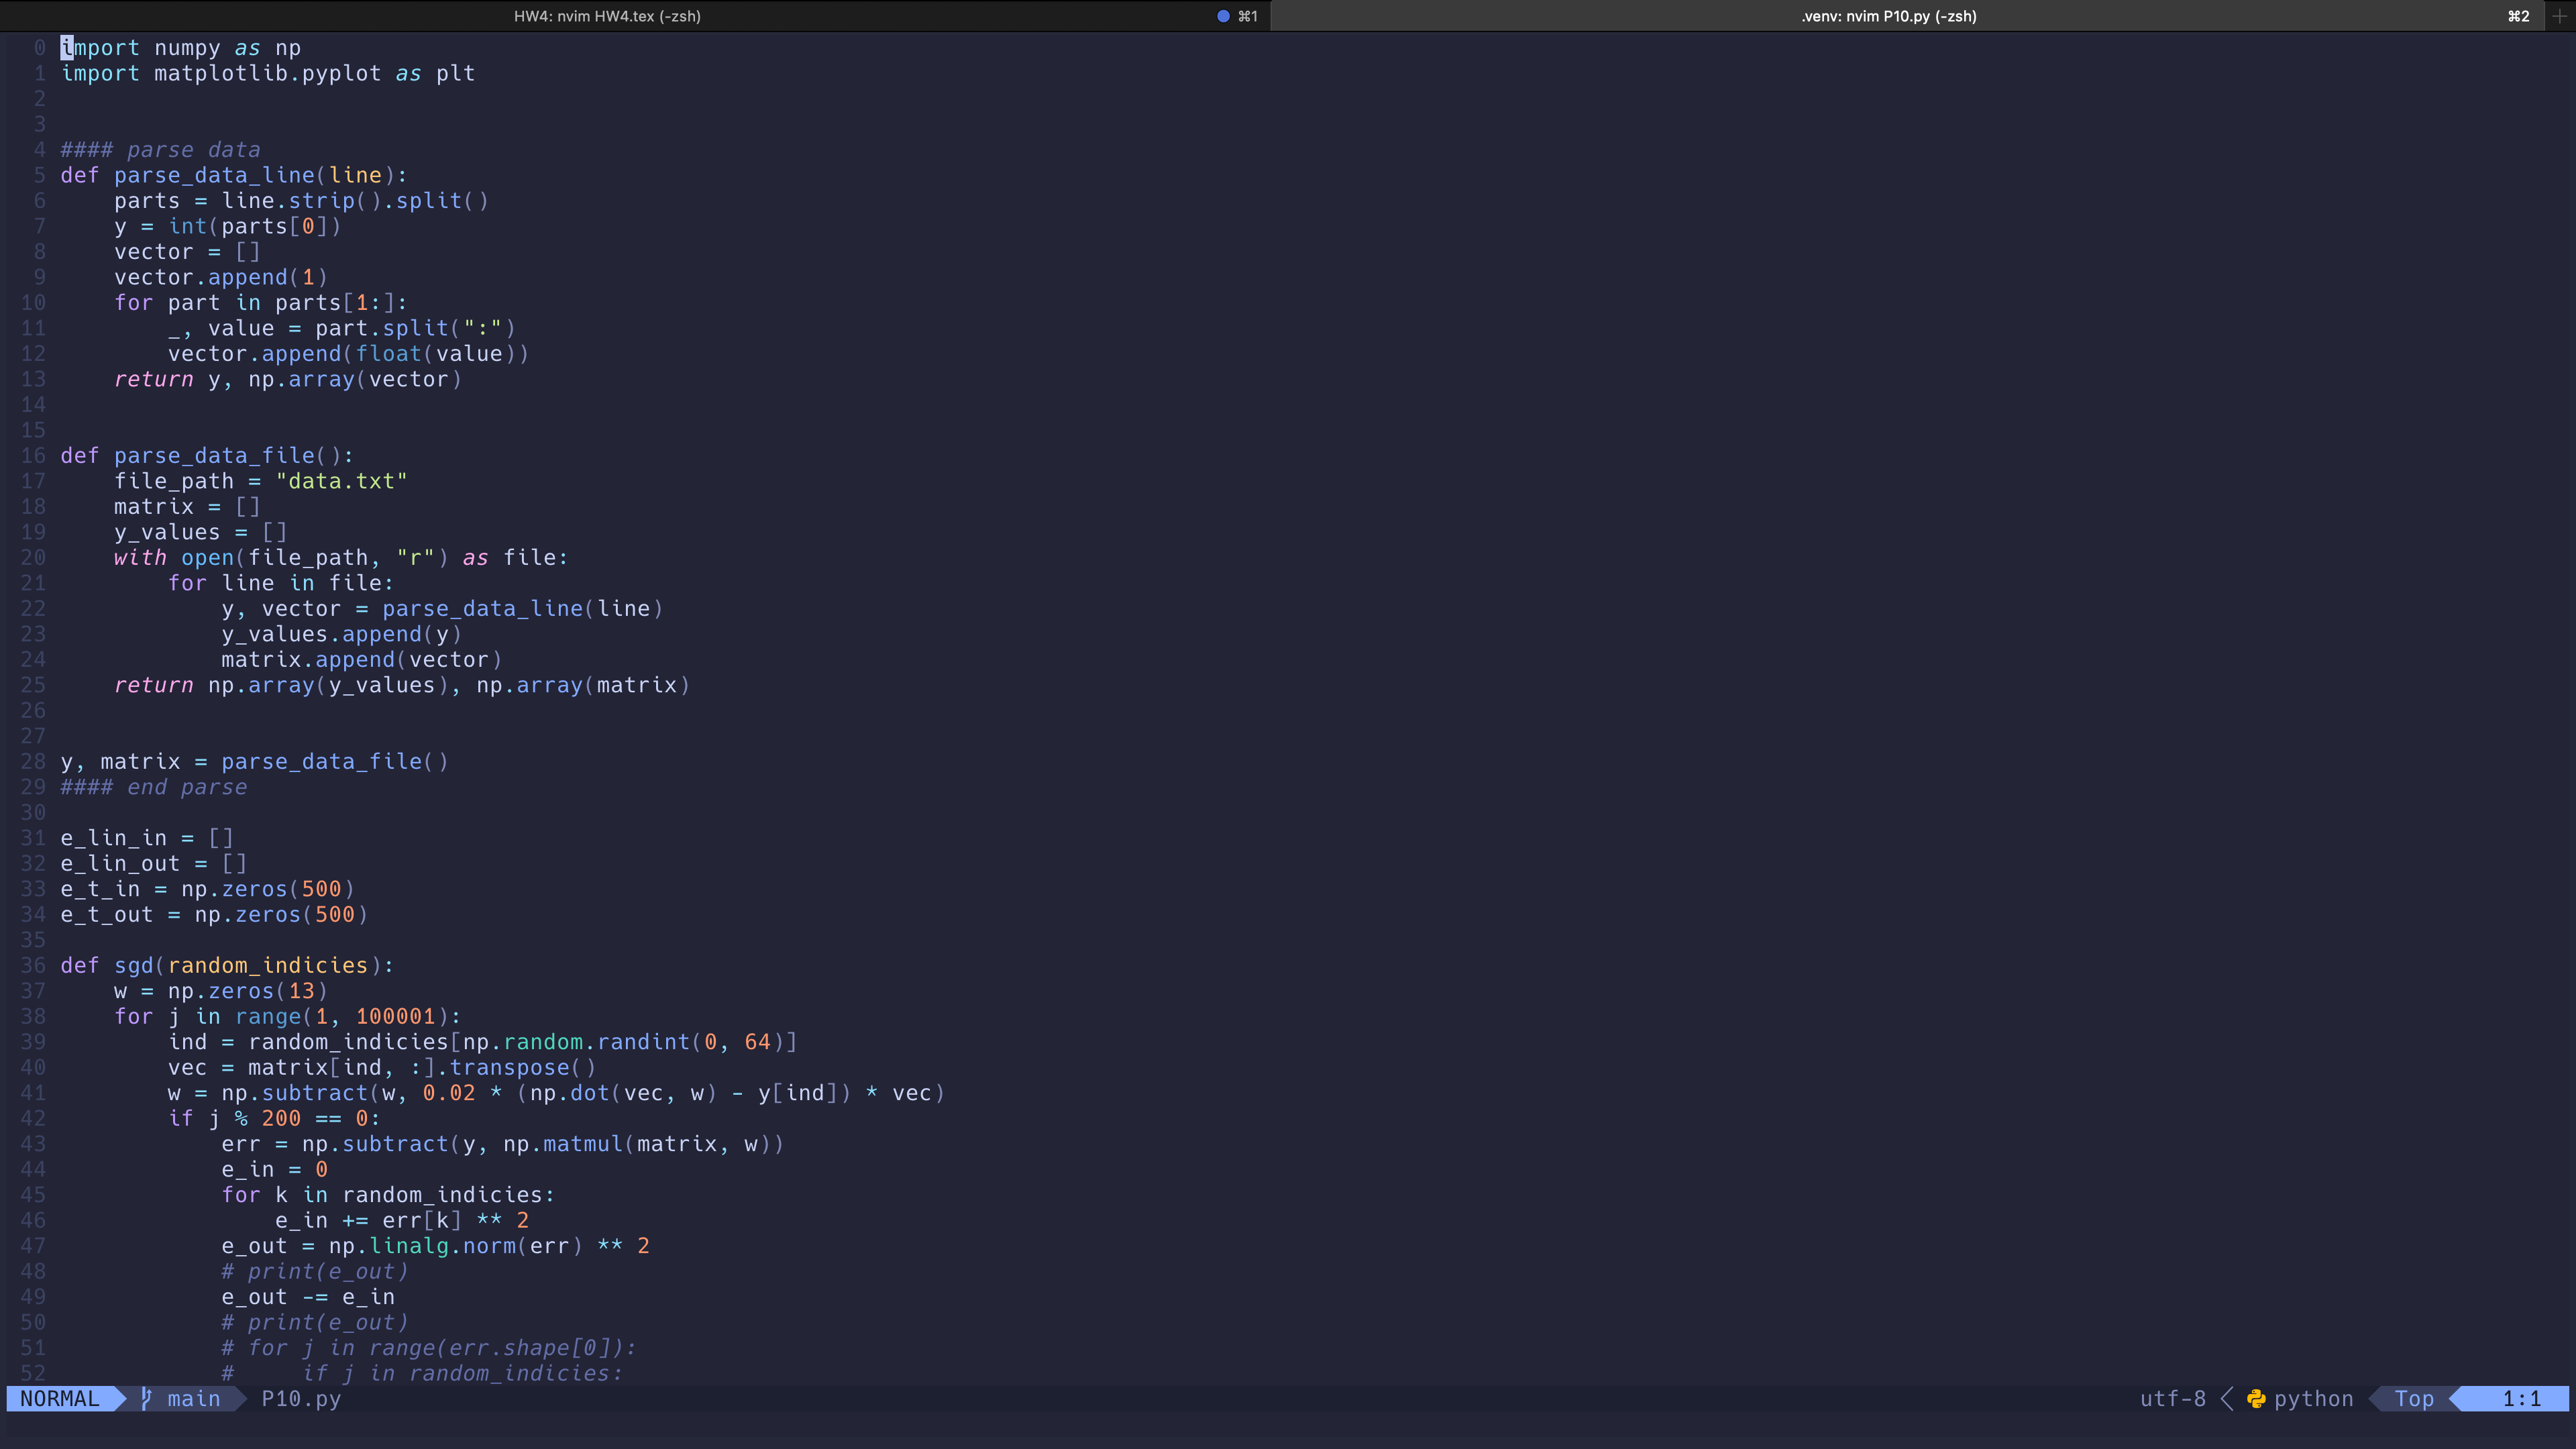
\includegraphics[width = \textwidth]{P10snap.png} \\
\newpage
\section*{11}
Figure: \\
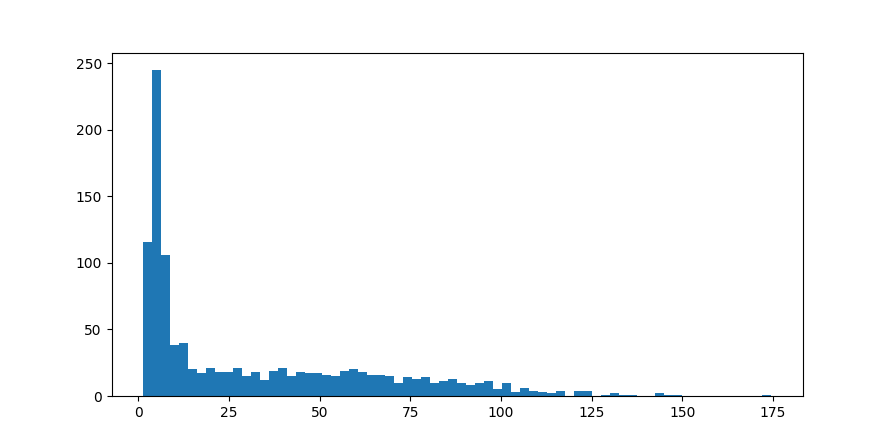
\includegraphics[width = \textwidth]{P11_fig_2.png}
\textbf{The average value of $E^{sqr}_{in}(\vb{w}_{lin}) - E^{sqr}_{in}(\vb{w}_{poly})$ is 32.45148423777838 } \\ 
\par
This figure is the histogram for $E^{sqr}_{in}(\vb{w}_{lin}) - E^{sqr}_{in}(\vb{w}_{poly})$, the horizontal axis is the value of $E^{sqr}_{in}(\vb{w}_{lin}) - E^{sqr}_{in}(\vb{w}_{poly})$, and the vertical axis is the number of times a value happens in the 1126 experiments (call this "frequency" in the following context). \\ 
We see that $E^{sqr}_{in}(\vb{w}_{lin}) - E^{sqr}_{in}(\vb{w}_{poly})$ mostly fall between $0$ and $10$, as the frequency is high in this range. The frequency drops rapidly at about $E^{sqr}_{in}(\vb{w}_{lin}) - E^{sqr}_{in}(\vb{w}_{poly}) = 10$, after the rapid drop, $E^{sqr}_{in}(\vb{w}_{lin}) - E^{sqr}_{in}(\vb{w}_{poly})$ decreases slowly, the largest value is slightly less than $150$. \\ 
The histogram and the average value of $E^{sqr}_{in}(\vb{w}_{lin}) - E^{sqr}_{in}(\vb{w}_{poly})$ implies that the homogeneous polynomial transform does indeed result in a $E_\text{in}$ gain. (which is in fact a decrease in $E_\text{in}$, but can be seen as a gain in the ability to fit the training set judging by $E_\text{in}$). Furthermore, compared with the average value of $E_\text{in}(\vb{w}_{lin})$ in P10, which is about $35$ (see the light-blue horizontal line at the bottom), the $E_{in}$ gain ($\approx 32.5$) is quite significant. This further shows that the polynomial transform reduces $E_{in}$ effectively. This is because by allowing a more complicated model, the classifier can fit the $N = 64$ training data vectors better.  \\
\newpage
Code snapshot: \\ 
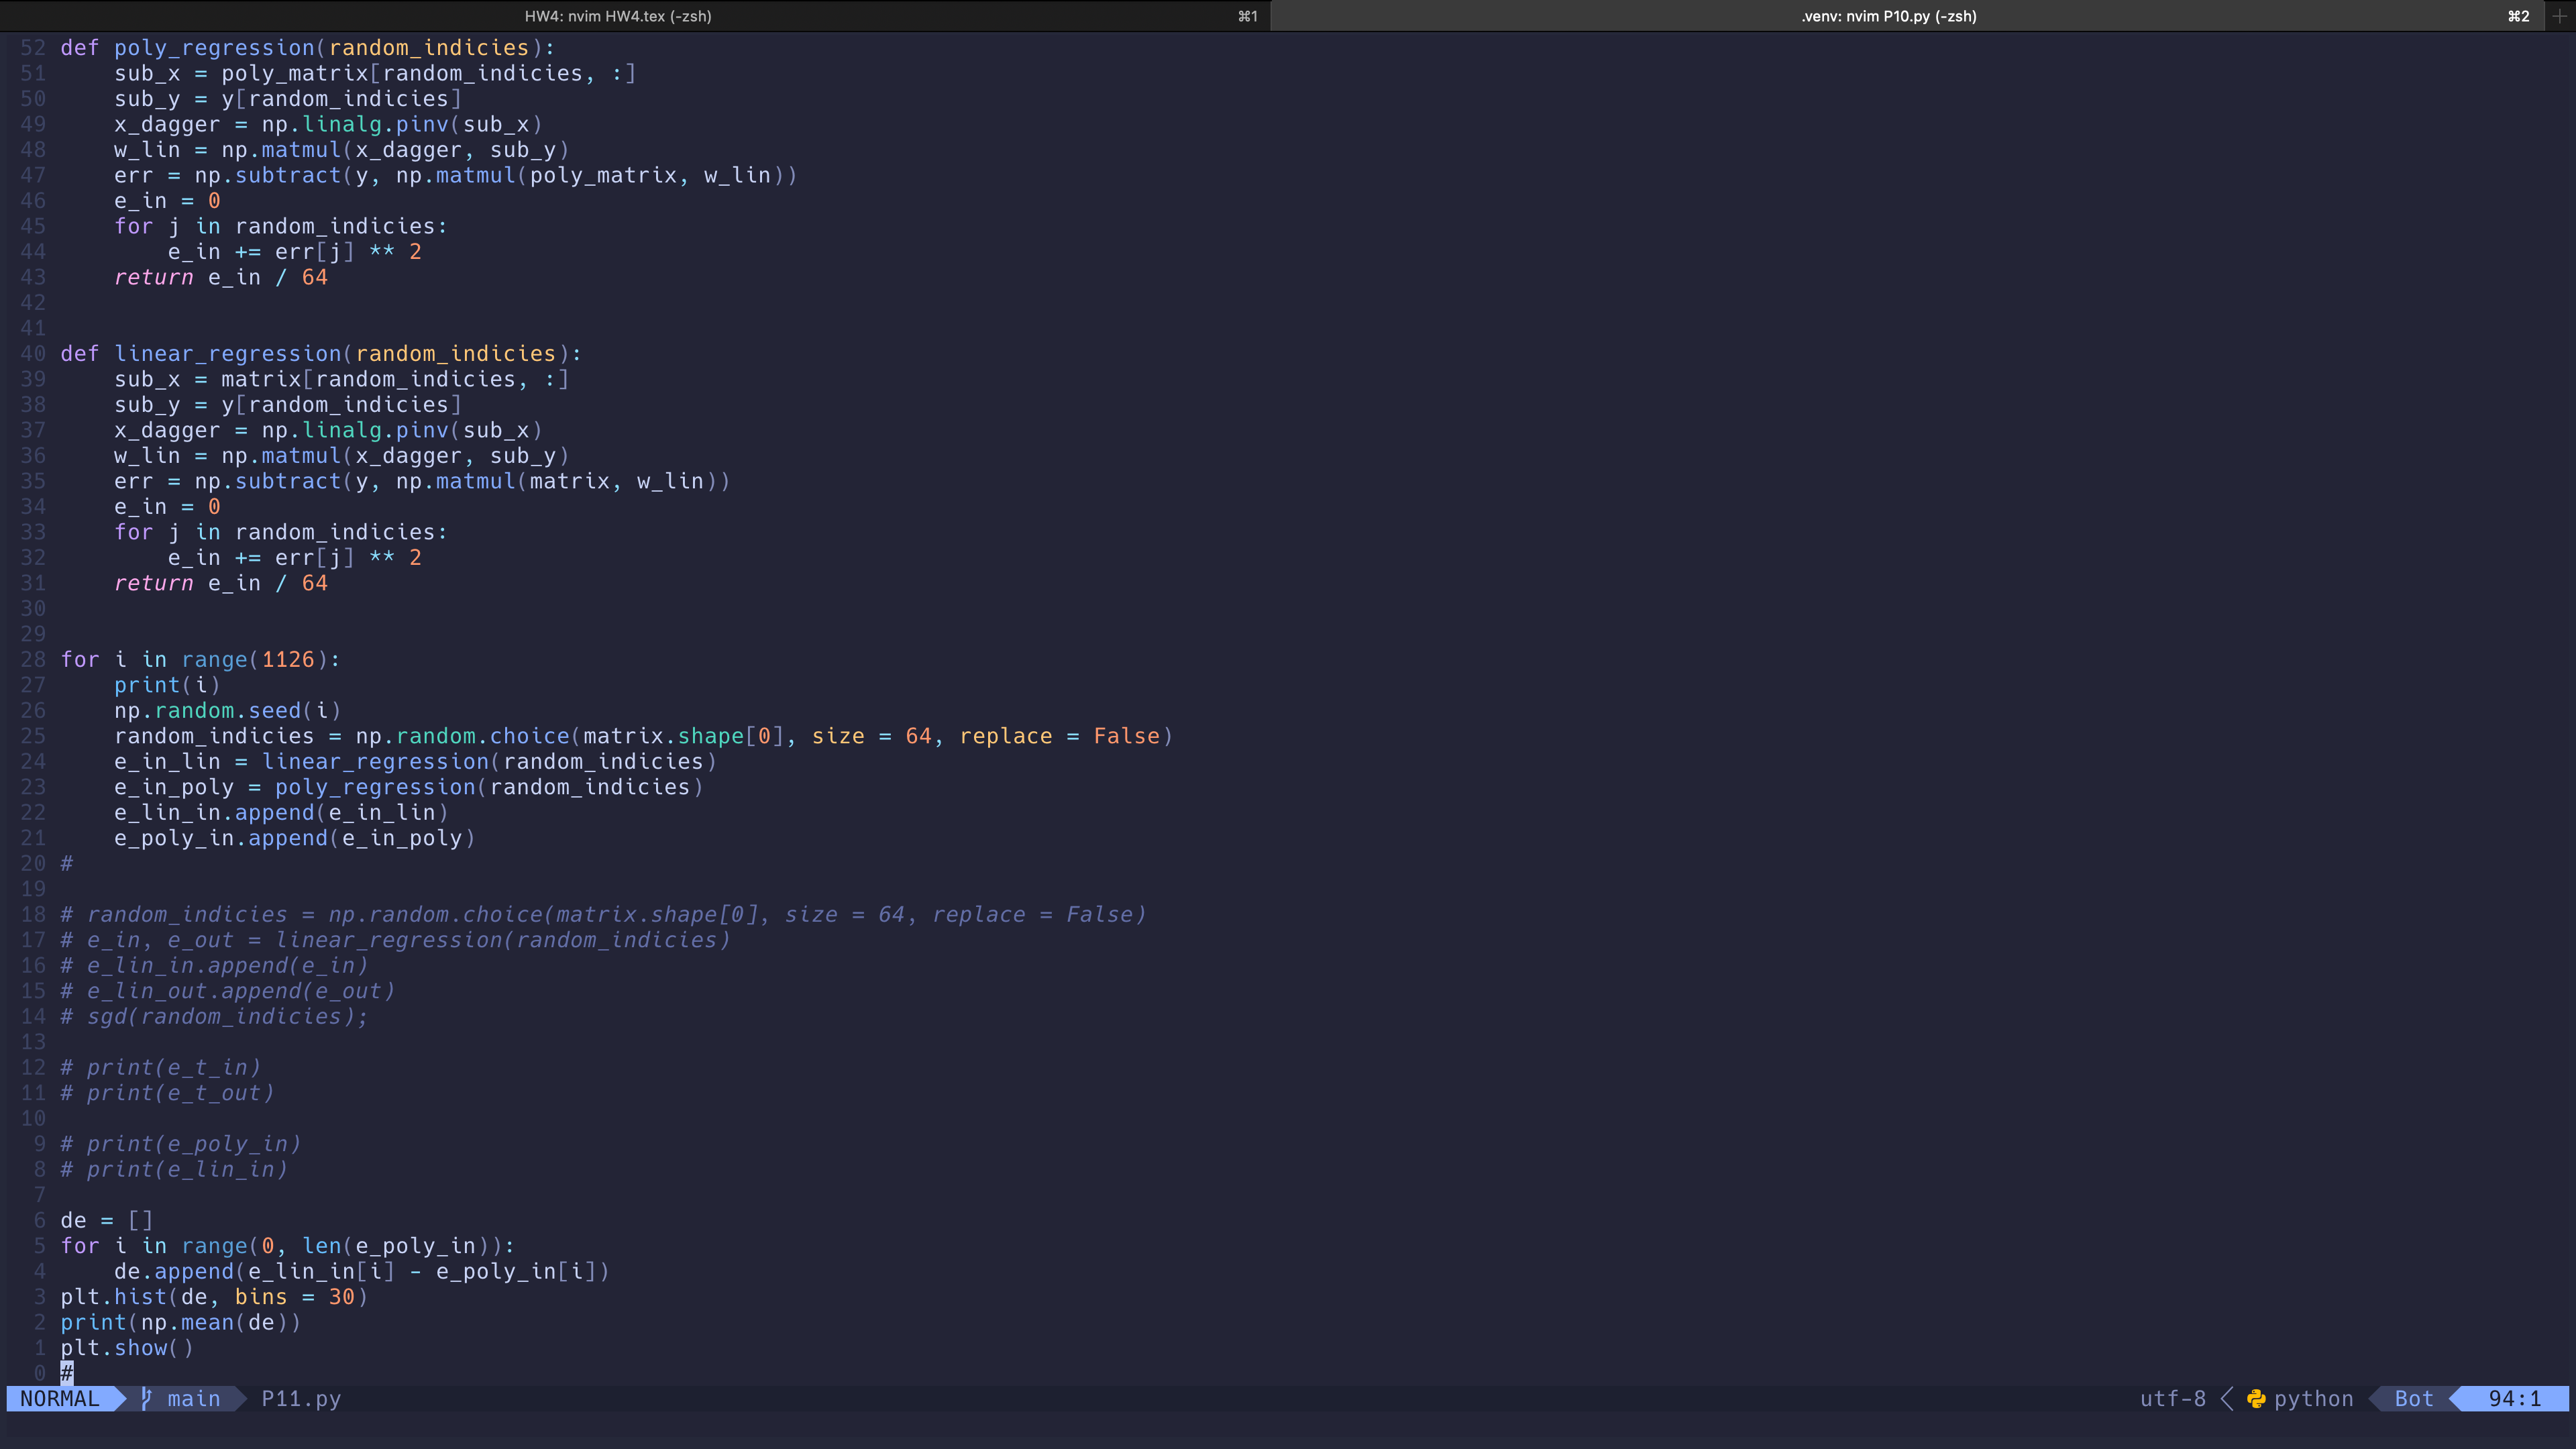
\includegraphics[width = \textwidth]{P11snap.png} \\ 
\newpage
\section*{12}
Figure: \\ 
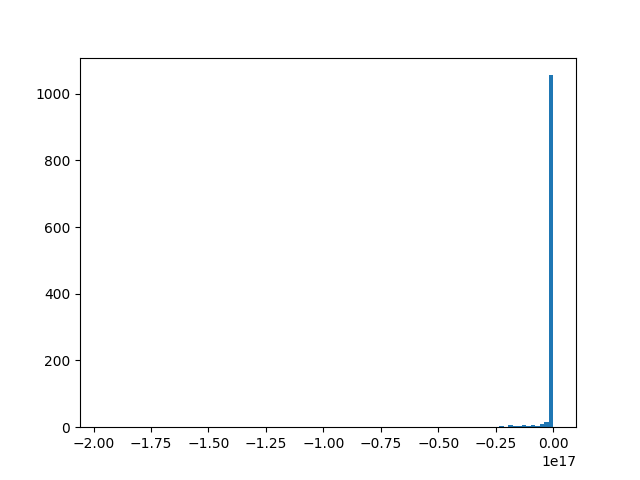
\includegraphics[width = \textwidth]{P12.png} \\
\textbf{The average value of $E^{sqr}_{out}(\vb{w}_{lin}) - E^{sqr}_{out}(\vb{w}_{poly})$ is -1051028513192239.2} \\ 
\par
This figure is the histogram of $E^{sqr}_{out}(\vb{w}_{lin}) - E^{sqr}_{out}(\vb{w}_{poly})$, the horizontal axis is the value of $E^{sqr}_{out}(\vb{w}_{lin}) - E^{sqr}_{out}(\vb{w}_{poly})$, and the vertical axis is the number of times a value happens in the 1126 experiments. \\
We see that $E^{sqr}_{out}(\vb{w}_{poly}) - E^{sqr}_{out}(\vb{w}_{lin})$ is huge, which implies that $E^{sqr}_{out}(\vb{w}_{poly})$ is far greater than $E^{sqr}_{out}(\vb{w}_{lin})$. \\ 
Together with the result in P11, we can see that adopting the polynomial transform in this problem makes classifying performance a lot worse. This is because the polynomial transform allows a more complicated model, and although $E_\text{in}$ is decreased, the classifying performance is worse due to the hazard of overfitting. \\ 
To conclude, the linear regression with the polynomial transform in this problem results in a bad learning model. (compared with direct linear regression)
\newpage
Code snapshot: \\ 
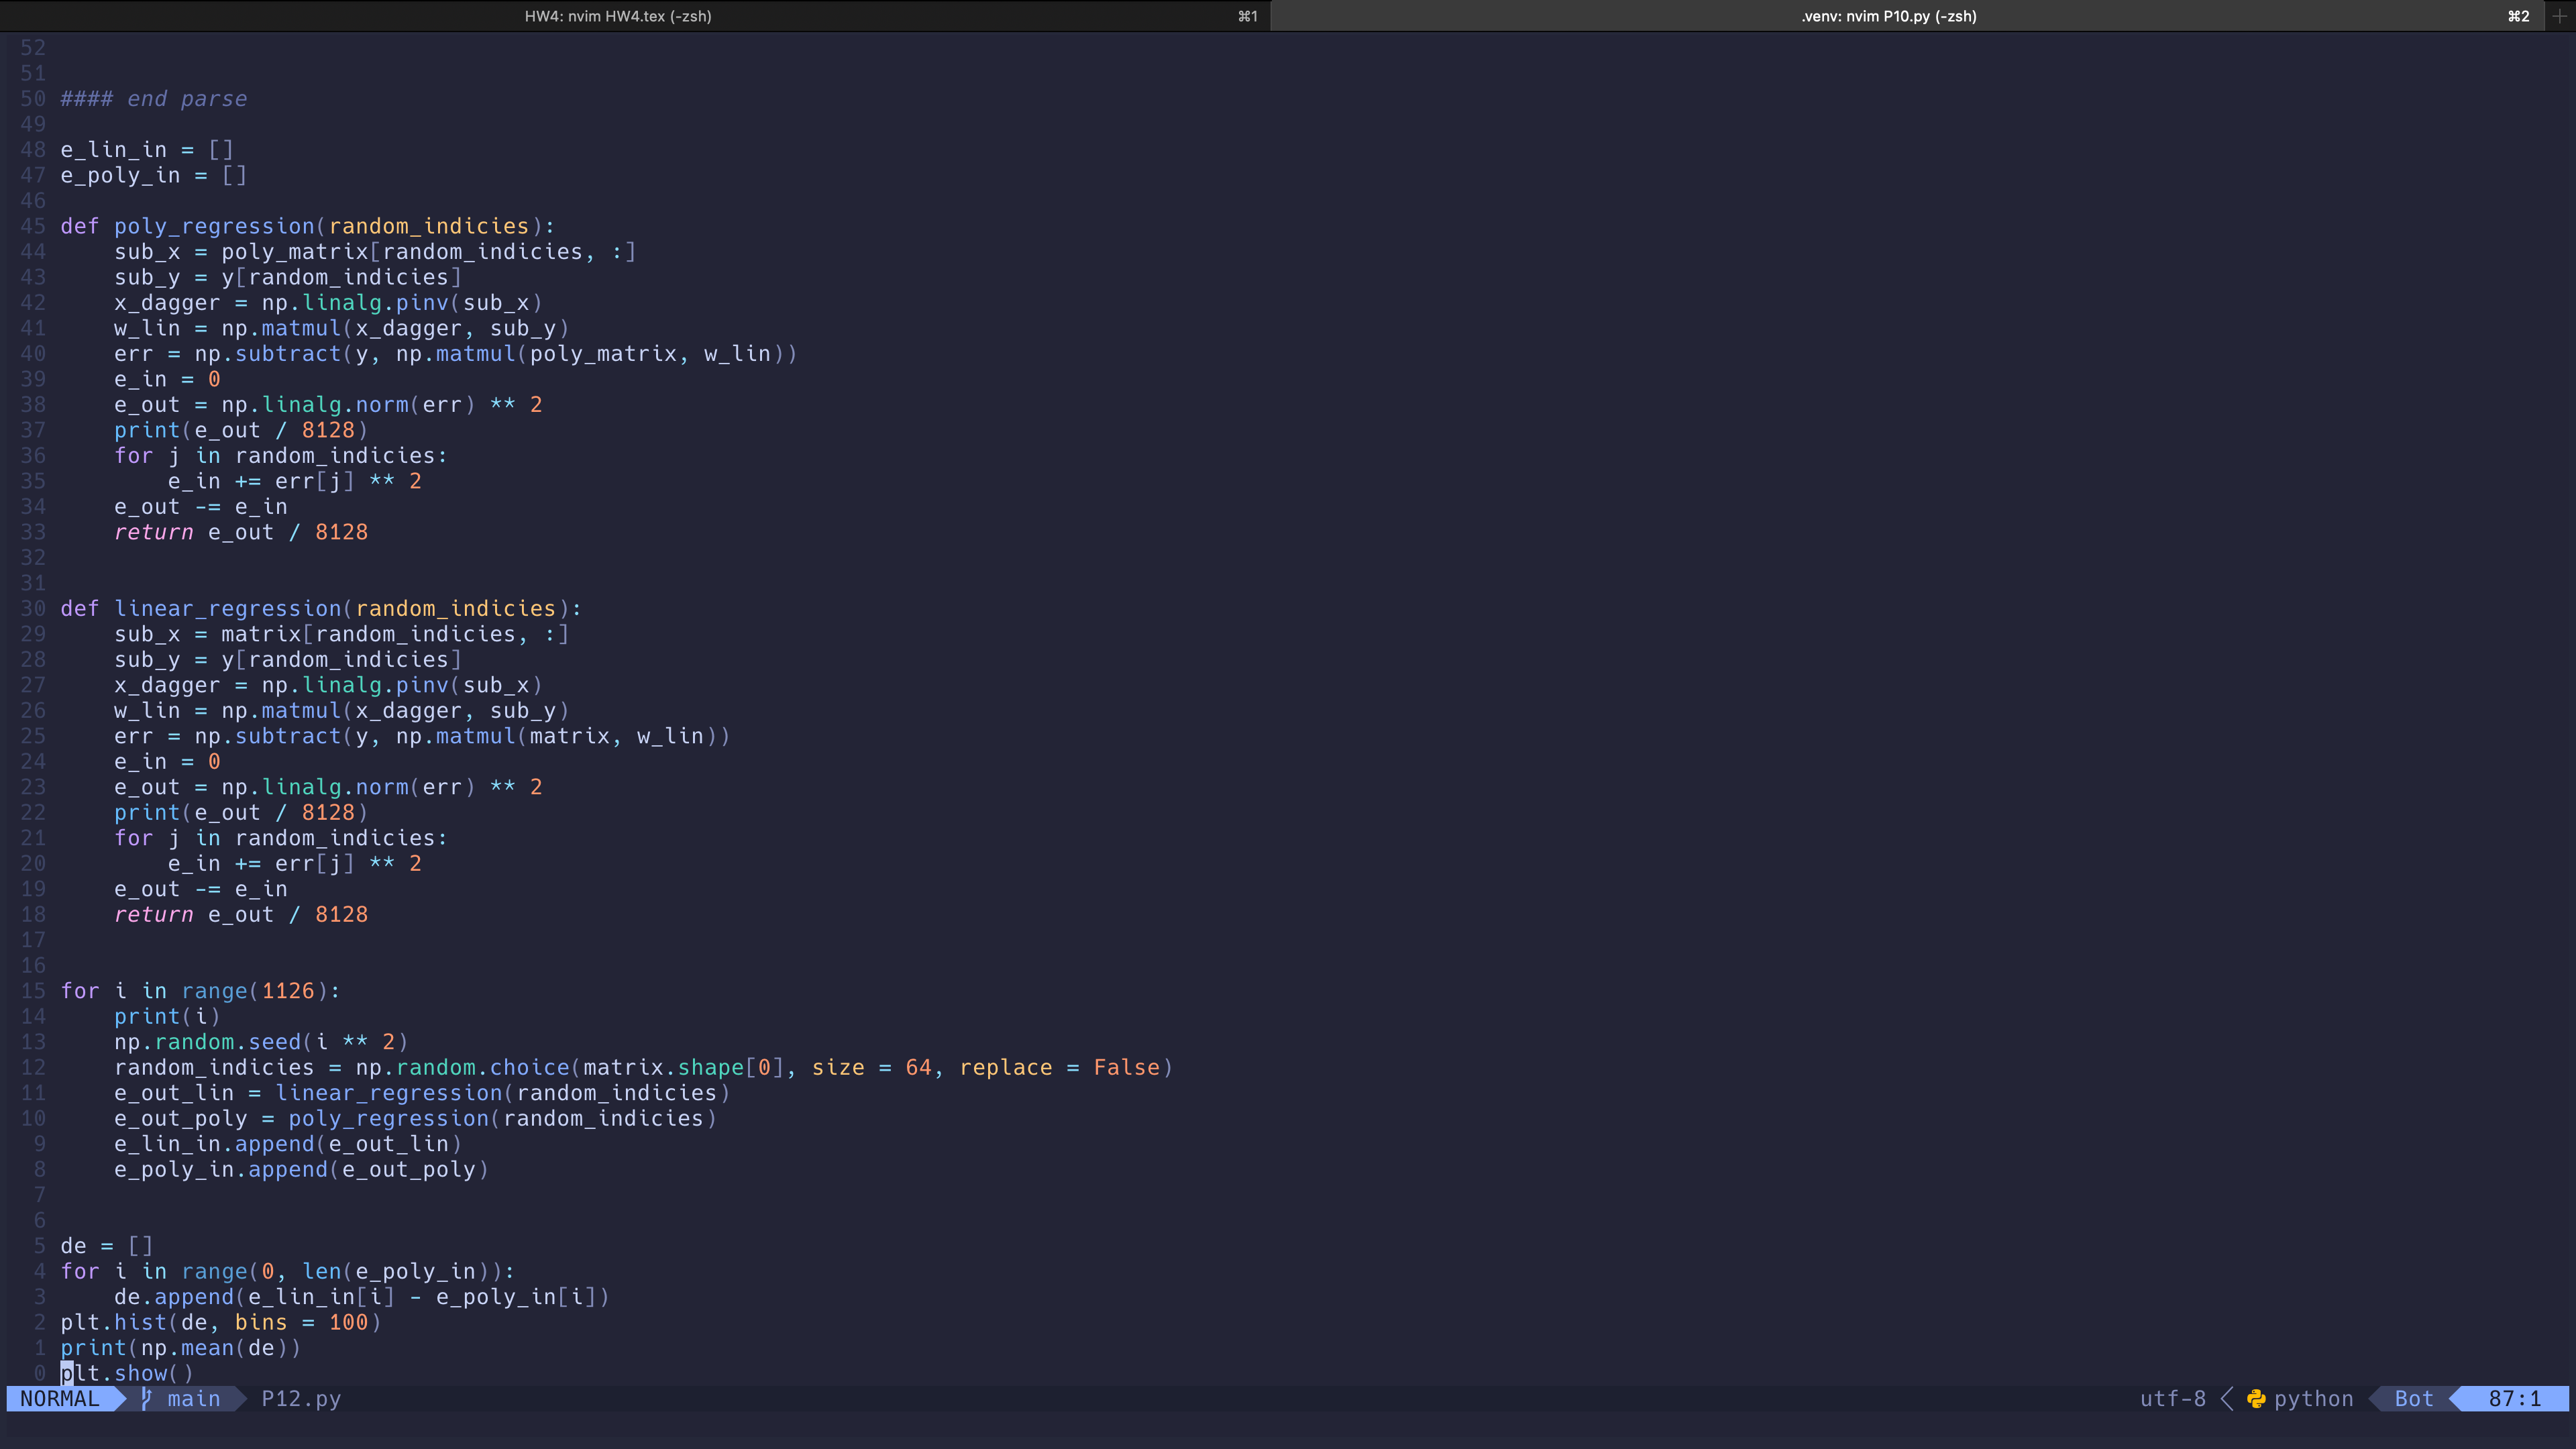
\includegraphics[width = \textwidth]{P12snap.png}
\newpage
\section*{13}
Notice that 
\begin{align*}
  \text{sign}\left(w_0 + \sum^d_{i = 1}w_ix_i\right) &= \text{sign}\left(\exp\left(w_0 + \sum^d_{i = 1}w_ix_i\right) - 1\right) \\ 
  &= \text{sign}\left(-e^{-w_0} + \prod^d_{i = 1}(\exp(x_i))^{w_i}\right)
\end{align*}
\par 
Therefore we see that $h_{\vb{w}}(\vb{x}) = \tilde{h}_{\vb{u}}(\vb{x}^\prime)$ if we let 
\begin{align*}
  u_0 &= -e^{-w_0} \\ 
  u_i &= w_i \quad i = 1, 2,\dots,d \\ 
  x^\prime_i &= \exp(x_i) - 1 \\
\end{align*}
Hence if there exist $n$ data vectors shattered by $\mathcal{H}_1$, we can find a corresponding set of $n$ data vectors that is shattered by $\mathcal{H}_2$, which implies that $d_{vc}(\mathcal{H}_1) \leq d_{vc}(\mathcal{H}_2)$. \\
\par
We can also see that $h_{\vb{w}}(\vb{x^\prime}) = \tilde{h}_{\vb{u}}(\vb{x})$ if we let
\begin{align*}
  x^\prime_i &= \ln(1 + \abs{x_i}) \\ 
  w_0 &= 
  \begin{cases}
    -\ln(-u_0) & u_0 < 0 \\ 
    1 & u_0 \geq 0
  \end{cases} \\
  w_i &= 
  \begin{cases}
    u_i & u_0 < 0 \\ 
    0 & u_0 \geq 0 \\
  \end{cases}
  \quad i = 1, 2, \dots, d
\end{align*}
(Observe that $\tilde{h}_{\vb{u}}(\vb{x}) = +1$ if $u_0 \geq 0$) \\ 
Hence if there exist $n$ data vectors shattered by $\mathcal{H}_2$, we can find a corresponding set of $n$ data vectors that is shattered by $\mathcal{H}_1$, whcih implies that $d_{vc}(\mathcal{H}_2) \leq d_{vc}(\mathcal{H}_1)$. \\
Since $d_{vc}(\mathcal{H}_1) \leq d_{vc}(\mathcal{H}_2)$ and $d_{vc}(\mathcal{H}_2) \leq d_{vc}(\mathcal{H}_1)$, $d_{vc}(\mathcal{H}_2) = d_{vc}(\mathcal{H}_1)$, and the statement is disproved.


\end{document}


